\documentclass[a4paper]{article}
\usepackage{import}
\subimport{../}{preamble}
\begin{document}

\section{Derivation of the Normal Modes of a Spherical Metallic Nanoparticle}
%\newcommand{\pot}{\ensuremath{\varphi}}
\newcommand{\const}{\ensuremath{\lambda}}

The Laplace equation,
\begin{equation}
\nabla^2\pot = 0,
\end{equation}
describes the behaviour of an electrostatic potential, \pot. In a spherically symmetric system the Laplace equation is expanded into,
\begin{equation}
\nabla^2\pot = \frac{1}{r^2}\frac{\partial}{\partial r} \left( r^2 \frac{\partial\pot}{\partial r} \right) + \frac{1}{r^2\sin\theta}\frac{\partial}{\partial\theta} \left( \sin\theta \frac{\partial\pot}{\partial\theta} \right) + \frac{1}{r^2\sin^2\theta}\frac{\partial^2\pot}{\partial\phi^2} = 0.
\end{equation}
This can be solved by separating the variables such that $\pot(r,\theta\phi)=R(r)Y(\theta,\phi)$ giving two separate equations,
\begin{subequations}
\begin{align}
\frac{1}{R}\frac{d}{dr}\left(r^2\frac{dR}{dr}\right)&=\const, \label{eq:R} \\
\frac{1}{Y}\frac{1}{\sin\theta}\frac{\partial}{\partial\theta}\left(\sin\theta\frac{\partial Y}{\partial\theta}\right) + \frac{1}{Y}\frac{1}{\sin^2\theta}\frac{\partial^2Y}{\partial\phi^2}&=-\const, \label{eq:Y}
\end{align}
where \const\ is an arbitrary constant required for both equations to sum to zero. Functions of the form of $Y(\theta,\phi)$ are considered spherical harmonics describing the angular component of a spherical system. Separating again to $Y(\theta,\phi)=\Theta(\theta)\Phi(\phi)$ leads to another two equations from \eqref{eq:Y},
\begin{align}
\frac{1}{\Phi}\frac{d^2\Phi}{d\phi^2}&=-m^2, \label{eq:Phi} \\
\const\sin^2\theta + \frac{\sin\theta}{\Theta}\frac{d}{d\theta}\left(\sin\theta\frac{d\Theta}{d\theta}\right)&=m^2, \label{eq:Theta}
\end{align}
\end{subequations}
where $m$ is another constant. \eqref{eq:Phi} has a solution $\Phi(\phi)=\e^{\pm im\phi}$. \eqref{eq:Theta} has solutions given by associated Legendre polynomials $\Theta(\theta)=P_l^m(\cos\theta)$ of degree $l$ and order $m$, restricting $-l \leq m \leq l$. \eqref{eq:R} then has a solution $R = A_lr^l + B_lr^{-(l+1)}$. Combining these into the electrostatic potential leads to a general solution,
\begin{equation}
\pot_{l,m_l}(r,\theta,\phi) = \sum_{l=0}^{l=\infty} \sum_{m_l=-l}^l [ A_lr^l + B_lr^{-(l+1)} ] P_l^m (\cos\theta) e^{i m_l\phi}.
\end{equation}

\begin{figure}[h]
\centering
\includegraphics[width=0.7\textwidth]{figures/spherical_harmonics}
\caption*{Image taken from wikipedia}
\label{fig:spherical_harmonics}
\end{figure}

The spherical harmonics set the charge distributions of the normal modes of oscillation in a \gls{mnp}.

%\section{Mie Theory}

%Mie theory \cite{mie1908} is...

%\begin{figure}[h]
%\centering
%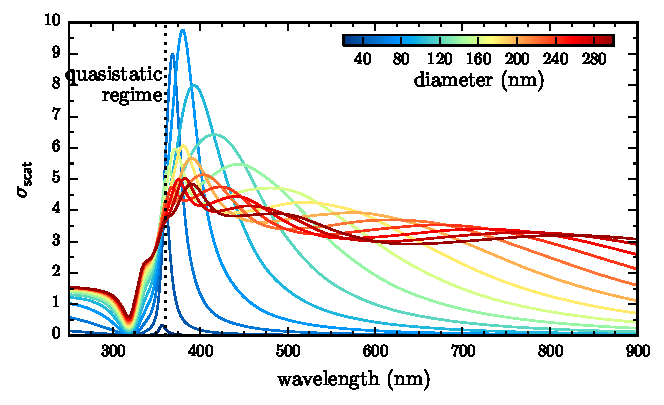
\includegraphics{figures/mie_scattering_ag}
%\caption[Mie scattering {\color{red}efficiencies/cross-sections} for AgNPs of increasing diameter]{\textbf{Mie scattering {\color{red}efficiencies/cross-sections} for AgNPs of increasing diameter.} The \SI{360}{nm} resonance position of the dipolar LSP mode of a AgNP in the quasistatic approximation is indicated by the dotted line. The resonance stays at \SI{360}{nm} until $d>\SI{60}{nm}$ then redshifts. The emergence of higher order modes following a similar behaviour is seen once $d>\SI{100}{nm}$.}
%\label{fig:mie_scattering_ag}
%\end{figure}

\section{Tip Modelling}

\begin{figure}[bt]
\subimport{./figures/}{tip_ellipsoidal_approximation.pdf_tex}
\caption*{\textbf{Ellipsoidal model for a sharp tip structure.} Tips have initially been modelled as spheres under the belief that only the apex radius dictated their properties. Ellipsoidal particles were modelled to attempt to analytically incorporate the finite length of the tip. Realistically the large length of the tip compared with the apex radius mean that such modelling is invalid and a plasmonic antenna model fails.}
\label{fig:tip_ellipsoidal_approximation}
\end{figure}

\section{Quantum Charge Transport}

One of main discussions of this work is the effect of quantum charge transport on plasmon coupling. Both quantum tunnelling and ballistic transport are qualitatively described in the main text for simplicity. The following section shows the relevant mathematical derivations of the conduction properties of metals resulting in the phenomena of quantum tunnelling and ballistic transport.

\subsection{Quantum Electron Tunnelling}

\subsection{Ballistic Conduction}

A 1D constriction between two charge reservoirs of length $L$ and width $W$ can be described as either diffusive if $l,l_\phi \ll L,W$, ballistic if $l,l_\phi \gg L,W$, or quasi-ballistic if inbetween, where $l$ and $l_\phi$ are the mean free path and phase coherence length, respectively. Conductance in the diffusive regime is as classically expected, $G=W\sigma_{2D}/L$. In the ballistic regime, however, it inherits quantum properties as is thus given by the Landauer formula,
\begin{equation} G=\frac{2e^2}{h}T(E_F), \end{equation}
where $T(E_F)$ is the transmission coefficient of an electron at the Fermi level. This is derived from the current flowing through a barrier between two biased reservoirs, whereby the Fermi levels are related via $E_{F,L} - E_{F,R} = eV$. The leftwards current through a barrier is given by,
\begin{equation}
	I_L = 2e \int_0^\infty f(E(k), E_{F,L}) v(k) T(k) \frac{dk}{2\pi},
	\label{eq:left_ballistic_current}
\end{equation}
where $f(E, E_F)$ is the Fermi-Dirac function and the wavevector of an electron can be related to its energy via $dE = \hbar v dk$. Converting \eqref{eq:left_ballistic_current} to an energy basis and adding the rightwards current yields,
\begin{equation}
	I_L = \frac{2e}{h} \int_{E_{L}}^\infty \left[ f(E(k), E_{F,L}) - f(E(k), E_{F,R}) \right] T(E) dE.
	\label{eq:ballistic_barrier_current}
\end{equation}
In the small bias limit%
\footnote{Large biases are ignored}
the Fermi-Dirac function is expanded as a Taylor series into,
\begin{equation}
	f(E(k), E_{F,L}) - f(E(k), E_{F,R}) \approx eV \frac{\delta f(E(k), E_F)}{\delta E_F}.
\end{equation}
Substituting this into \eqref{eq:ballistic_barrier_current} yields the integral,
\begin{equation}
	I_L = \frac{2e^2V}{h} \int_{E_{L}}^\infty \left[ -\frac{\delta f}{\delta E} \right] T(E) dE.
\end{equation}
At low temperatures $\delta f/\delta E \rightarrow \delta(E-E_F)$ and the integral evaluates to,
\begin{equation}
	I_L = \frac{2e^2V}{h}T(E_F),
\end{equation}
from which the conductance $G=I/V$ is derived to be,
\begin{equation}
		G = \frac{2e^2}{h}T(E_F).
\end{equation}
With the barrier still in place this corresponds to a tunnelling conductance with $T(E_F)<1$. The point at which the barrier disappears ($E_{barrier} = E_F$) gives rise to $T(E) = 1$ and opens up a single quantised conductance channel. Adding additional $n$ sub-bands into the constriction continues to increase the conductance by its quantum, $2e^2/h$, and thus the conductance of a 1D \emph{conductive} junction can be expressed as,
\begin{equation}
	G = \frac{2e^2}{h}n.
\end{equation}

\end{document}

